\documentclass{llncs}
\usepackage[portuguese]{babel}  % Portuguese
\usepackage[utf8]{inputenc}
\usepackage{graphicx}
\usepackage{caption}
\usepackage{subcaption}
\usepackage{float}              % improve figures & tables floating
\usepackage{mathrsfs}
\usepackage{array}

\graphicspath{{figures/}}
\captionsetup{compatibility=false}
\setlength{\intextsep}{7pt}

%
\begin{document}
\pagestyle{headings}  % switches on printing of running heads
\title{Visage \\ Impacto dos Filtros de Abstração no Reconhecimento Facial em Imagens}

\author{Pedro Pontes\inst{1}, Filipe Coelho\inst{1,3} e Cristina Ribeiro\inst{2,3}}

\institute{Laboratório SAPO/U.Porto \\
\email{ei08091@fe.up.pt} \and
INESC Tecnologia e Ciência \\
\email{filipe.coelho@fe.up.pt}
\and Departamento de Engenharia Informática - Universidade do Porto \\
\email{mrc@fe.up.pt}}

\maketitle

\begin{abstract}
O reconhecimento facial em imagens constitui uma área de investigação em aberto, principalmente se considerarmos situações de captura de imagens não controladas. Os filtros de abstração atuam como ferramentas de remoção de informação redundante existente nas imagens. Foi desenvolvido um sistema de reconhecimento facial de personalidades, baseado em código aberto, onde é utilizada a abstração de imagens juntamente com tarefas de pré-processamento paralelas, de forma a analisar o seu impacto no processo de reconhecimento. A avaliação foi efetuada com recurso à coleção de imagens \textit{Labeled Faces in the Wild}, sob duas perspetivas, \textit{Closed-set Identification} e \textit{Image Retrieval}, e utilizando nove cadeias de pré-processamento de imagens distintas.
Os resultados demonstram que a aplicação de filtros de abstração no processo de reconhecimento resulta no compromisso entre a diminuição dos requisitos de armazenamento das imagens e a ligeira redução da eficácia da identificação. A deteção e segmentação das faces presentes nas imagens revelou ser a etapa de pré-processamento com maior importância para um reconhecimento eficaz. O desempenho foi avaliado através dos algoritmos \textit{Eigenfaces}, \textit{Fisherfaces} e \textit{Local Binary Patterns Histograms}, tendo o último revelado o melhor desempenho em termos globais.
\end{abstract}

\section{Introdução}
A sociedade atual caracteriza-se pelo constante fluxo de informação a que os seus indivíduos estão expostos, assistindo-se a um crescimento acelerado na produção de conteúdos multimédia, tendo em conta os meios de transmissão de informação digital. Neste contexto, torna-se importante o desenvolvimento de novas metodologias que possibilitem a categorização, organização e pesquisa por parte dos utilizadores destes conteúdos \cite{Datta2008}, representando o reconhecimento facial automático em imagens um papel importante a esse nível.

Ao longo dos últimos 20 anos o reconhecimento facial em imagens sofreu uma evolução notável. Em condições de captura de imagens controladas, nomeadamente ao nível da pose, iluminação e expressões faciais, considera-se mesmo que o problema de verificação 1:1, onde se verifica se existe uma correspondência entre a pessoa representada na imagem e a identidade fornecida, se encontra praticamente resolvido, uma vez que as taxas de reconhecimento atingidas são satisfatórias para a grande maioria das aplicações \cite{Li2011}. Contudo, o problema de reconhecimento facial automático ainda se encontra longe de ser um problema totalmente resolvido. Em cenários onde as condições de captura de imagens não são controladas, a identificação das entidades representadas nas imagens é ainda uma área de investigação em aberto \cite{Li2011,Pinto2009}.

Por seu lado, a abstração de imagens dota os artistas de novas ferramentas de transmissão de informação, tendo como objetivo, melhorar eficácia da comunicação visual. Os filtros de abstração permitem remover informação não essencial de uma imagem, dando apenas destaque à mensagem a transmitir. A aplicação de filtros de abstração de imagens na recuperação de informação multimédia, nomeadamente no âmbito da da ilustração automática de texto, tem a potencialidade de melhorar a informação retornada, assim como reduzir significativamente as necessidades de processamento e armazenamento das imagens \cite{Coelho:2012:IAC:2260641.2260676}. 

Neste artigo, encontra-se descrito  o sistema de reconhecimento facial automático em imagens Visage e a avaliação efetuada ao impacto da abstração e outras tarefas de pré-processamento utilizadas no processo de reconhecimento.

\section{Sistema de Reconhecimento Facial}

\subsection{Visão Geral}
A criação do sistema de reconhecimento facial Visage teve como principal objetivo o desenvolvimento de um sistema automático de reconhecimento facial em imagens, baseado em código aberto, que permita analisar qual o impacto da abstração de imagens e outras tarefas de pré-processamento no processo de reconhecimento. Com o sistema desenvolvido pretende-se ainda a criação de uma base sólida que permita o desenvolvimento de futuras aplicações que tirem partido do reconhecimento facial automático no seu funcionamento, como por exemplo, aplicações na área de \textit{image retrieval} e contribuir para existência de um maior número de soluções de código aberto deste tipo. De seguida encontram-se descritas as principais etapas de processamento no sistema.

\subsection{Pré-processmento}\label{sec:pre-processamento}

A primeira tarefa desempenhada pelo sistema criado consiste no pré-processamento das imagens. Para esse fim foram desenvolvidas as seguintes sub-tarefas de pré-processamento:
\begin{enumerate}
\item \textbf{Deteção e Corte da Face:} Tem como objetivo determinar a zona da imagem onde se encontra a face a identificar de forma a efetuar a segmentação da face da restante imagem. A sua implementação teve por base o uso de um \textit{boosted cascade classifier} treinado especialmente para a deteção de faces, disponível na biblioteca \textit{Open Source Computer Vision} (\textit{OpenCV}) baseado nos trabalhos de Viola e Jones \cite{Viola2001} e posteriores melhorias introduzidas por Lienhart \textit{et al.} \cite{Lienhart2003}.

\begin{figure}[t]
  \centering
    \leavevmode
    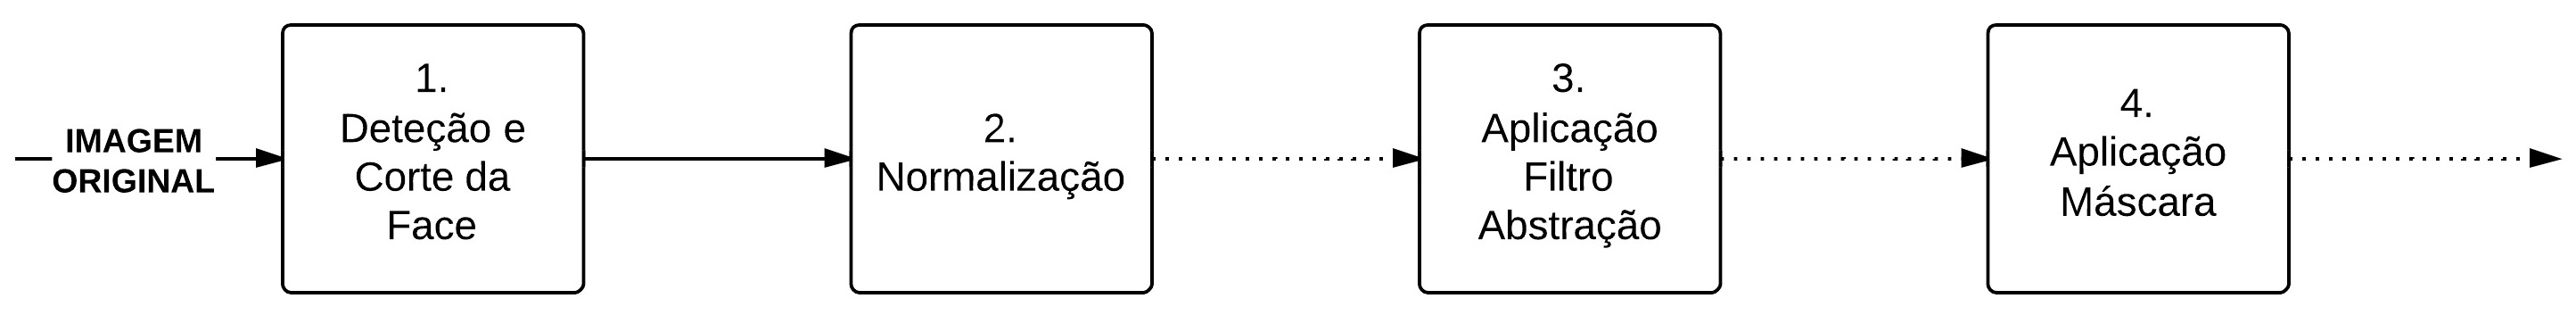
\includegraphics[width=1\textwidth]{PreProcessamentoVisage}
    \caption{Tarefas de pré-processamento utilizadas na avaliação do sistema Visage.}
    \label{fig:preprocessamento}
\end{figure}

\item \textbf{Normalização:} Permite efetuar a normalização do contraste da imagem recorrendo a três técnicas distintas. A primeira é designada \textit{Contrast Stretching} e consiste em alargar a gama de valores utilizados para mapear a intensidade da imagem através de um mapeamento linear dos valores originais para uma gama de intensidade entre 0 e 255. A segunda técnica, Equalização do Histograma, consiste num mapeamento do histograma da imagem utilizando a função de distribuição acumulada (\textit{cumulative distribution function}) de forma a que o histograma resultante se aproxime de uma distribuição mais alargada e idealmente de intensidade uniforme \cite{Bradski2008}. A última técnica, \textit{Contrast limited adaptive histogram equalization} (\textit{CLAHE}), procura ultrapassar as limitações da técnica de equalização do histograma ao ter em consideração a intensidade de um conjunto de píxeis e dos seus vizinhos para a normalização em vez de considerar toda a imagem. Para além disso, esta última abordagem considera ainda um limite para o qual a equalização é realizada, evitando assim  um mapeamento demasiado agressivo \cite{Reza2004}. Todas as técnicas de normalização foram integradas no sistema Visage utilizando como base a biblioteca \textit{OpenCV}.

\item \textbf{Aplicação de Filtro de Abstração:} Efetua a abstração da imagem com recurso a um dos três filtros de abstração disponíveis, gaussiano, bilateral e Kuwahara anisotrópico. A aplicação de um filtro gaussiano é a uma técnica tipicamente aplicada no processamento de imagem  e computação gráfica para suavizar imagens \cite{373563} e corresponde ao menor nível de abstração dos três filtros utilizados. O filtro bilateral foi originalmente proposto por Tomasi e Manduchi \cite{Tomasi1998} e caracteriza-se por suavizar as zonas com menor contraste da imagem enquanto preserva os limites de maior contraste. O filtro Kuwahara anisotrópico é uma generalização do filtro Kuwahara original que remove alguns dos artefactos originados na aplicação do filtro original através da adaptação da escala e orientação do filtro à estrutura local da imagem \cite{Kyprianidis2009}. Os filtros gaussiano e bilateral, foram utilizados com recurso à implementação existente na biblioteca \textit{OpenCV} e o filtro Kuwahara anisotrópico, recorrendo à implementação efetuada por Kyprianidis \textit{et al.} \cite{Kyprianidis2009} do mesmo filtro.
\item \textbf{Aplicação de Máscara:} Aplicação de uma máscara elíptica sobre a imagem com o objetivo de remoção do fundo ainda existente após a deteção e segmentação da face e eventuais tarefas de pré-processamento realizadas.
\end{enumerate}

As sub-tarefas 2, 3 e 4 são opcionais e independentes entre si, existindo assim a possibilidade de não aplicar uma das sub-tarefas sem prejudicar as restantes.

\subsection{Treino e Identificação}\label{sec:treino-id}
À fase de pré-processamento seguem-se as fases de treino e identificação. Na fase de treino é fornecido um conjunto de imagens anotadas ao sistema e pretende-se que este crie uma base de conhecimento que permita proceder à identificação de novas imagens na fase de identificação. A fase de identificação corresponde à utilização do sistema com o intuito de identificar novas imagens. Ambas as fases foram implementadas com recurso ao módulo de reconhecimento facial \textit{FaceRecognizer}, da biblioteca \textit{OpenCV}, que permite o treino de um modelo de reconhecimento facial com os algoritmos \textit{Eigenfaces} \cite{Turk1991}, \textit{Fisherfaces} \cite{Belhumeur1997,Zhao1998} e \textit{Local Binary Patterns Histograms  (LBPH)} \cite{ahonen2004face}. O módulo \textit{FaceRecognizer} foi ainda estendido de forma a que para uma dada imagem fornecida ao sistema seja devolvida uma lista ordenada das $n$ entidades mais parecidas com essa imagem e não apenas a entidade mais parecida.

\section{Avaliação}
\subsection{Conjuntos de Teste} \label{sec:conjuntos}
A coleção \textit{Labeled Faces in the Wild (LFW)} \cite{Huang2007} é uma base de dados fotográfica concebida para o estudo do problema de reconhecimento facial, particularmente em situações onde as condições de captura das imagens não possuem restrições. Nesse sentido, as imagens que constituem a galeria caracterizam-se por possuir uma grande variabilidade, nomeadamente ao nível da pose, expressão, iluminação, etnia, idade, género, vestuário e qualidade da câmara com a qual foi efetuada a captura \cite{Huang2007}. Nesta biblioteca encontram-se representados 5749 indivíduos, ilustrados por 13233 imagens, no entanto apenas 1680 indivíduos possuem duas ou mais imagens na biblioteca. A cada imagem encontra-se também associada uma anotação textual, relativa ao nome da pessoa representada. Na avaliação de desempenho aqui reportada foi utilizada uma versão pré-alinhada da biblioteca LFW, designada LFW-a \cite{WHT:BMVC09:MOS}, de forma a remover um importante fator de variação de desempenho, mantendo a análise efetuada centrada no impacto dos filtros de abstração e restantes tarefas de pré-processamento utilizadas.

As avaliações de desempenho efetuadas no âmbito deste projeto, não se enquadram no paradigma de \textit{pair matching} para o qual a biblioteca LFW foi originalmente criada, pelo que se tornou necessário o desenvolvimento de novos conjuntos de teste, neste caso foram criados 4 conjuntos. Cada um dos conjuntos possui um total de 1180 imagens, correspondentes a amostras biométricas de 59 indivíduos (20 imagens por indivíduo). As 20 imagens de cada indivíduo incluídas em cada um dos conjuntos de testes variam conforme o conjunto e foram selecionadas aleatoriamente. Algumas imagens encontram-se presentes nos quatro conjuntos de teste criados, enquanto outras apenas estão presentes apenas num conjunto, fazendo um total de 1592 imagens diferentes.

Para cada conjunto foram ainda criados dois sub-conjuntos de dados. O primeiro conjunto, designado galeria de treino ($\mathscr{G}$), é constituído por 80\% das imagens de cada pessoa, as quais são utilizadas para o treino  do sistema de reconhecimento facial. O segundo conjunto, designado provas ($\mathscr{P}$), contém os restantes 20\% das imagens de cada pessoa, as quais são utilizadas para a avaliação do desempenho do reconhecimento. As imagens presentes nos sub-conjuntos $\mathscr{G}$ e $\mathscr{P}$ diferem de forma aleatória entre os quatro conjuntos criados, sendo que uma imagem pode pertencer à galeria de treino de um conjunto e às provas de outro.

\subsection{Galerias pré-processadas}
Na avaliação efetuada foram utilizadas quatro tarefas de pré-processamento sobre as imagens a reconhecer, sendo que para uma tarefa de pré-processamento podem existir várias opções disponíveis, como por exemplo para a abstração das imagens, onde três filtros diferentes podem ser utilizados. Foram criadas nove galerias de imagens, para a análise do impacto das diversas etapas de pré-processamento no reconhecimento facial. As galerias possuem todas as imagens contidas nos conjuntos de teste definidos na Secção \ref{sec:conjuntos}, diferenciando-se pelos passos de pré-processamento a que as imagens foram sujeitas. Na Tabela \ref{tab:colecoes} encontram-se sintetizadas as nove galerias criadas e as etapas de pré-processamento aplicadas em cada galeria. A Figura \ref{fig:galeriaspreprocessadas} apresenta um exemplo do estado da mesma imagem nas nove galerias pré-processadas.

\begin{table}[t]
	\centering
	\caption{Galerias criadas após pré-processamento.}
    \begin{tabular}{l|cccc}
    \hline\hline
    Designação & 1.Deteção e Corte   & 2.Normalização           & 3.Filtro Abstração & 4.Máscara \\
	\hline
    Original   &   -         & -                      & -                &   -      \\
    Cropped    & Sim         & -                      & -                &   -      \\
    Masked     & Sim         & -                      & -                & Sim      \\
    Normalized & Sim         & \textit{Contrast Stretching}& -           & Sim      \\
    Equalized  & Sim         & Equa. Histograma & -                & Sim      \\
    Clahe     & Sim         & \textit{CLAHE}         & -                & Sim      \\
    Bilateral  & Sim         & Equa. Histograma & Bilateral        & Sim      \\
    Gaussian   & Sim         & Equa. Histograma & Gaussian         & Sim      \\
    AKF         & Sim        & Equa. Histograma & Kuwahara Anisotropico & Sim \\
    \hline\hline
    \end{tabular}
	\label{tab:colecoes}
\end{table}

\begin{figure}[t]
        \centering
        \begin{subfigure}[b]{0.2\textwidth}
                \centering
                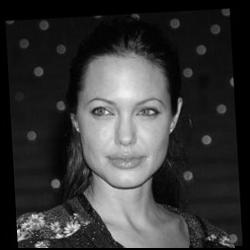
\includegraphics[width=\textwidth]{angelina/Angelina_Jolie_0006_original}
                \caption{Original}
                \label{fig:original-original} 
        \end{subfigure}%
        ~ ~
        \begin{subfigure}[b]{0.2\textwidth}
                \centering
                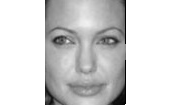
\includegraphics[width=\textwidth]{angelina/Angelina_Jolie_0006_cropped}
                \caption{Cropped}
                \label{fig:cropped} 
        \end{subfigure}
        ~ ~
        \begin{subfigure}[b]{0.2\textwidth}
                \centering
                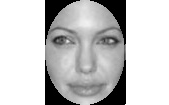
\includegraphics[width=\textwidth]{angelina/Angelina_Jolie_0006_masked}
                \caption{Masked}
                \label{fig:masked}
        \end{subfigure}%
%

        \begin{subfigure}[b]{0.2\textwidth}
                \centering
                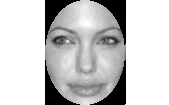
\includegraphics[width=\textwidth]{angelina/Angelina_Jolie_0006_normalized}
                \caption{Normalized}
                \label{fig:normalized} 
        \end{subfigure}
        ~ ~
        \begin{subfigure}[b]{0.2\textwidth}
                \centering
                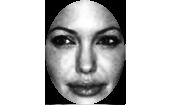
\includegraphics[width=\textwidth]{angelina/Angelina_Jolie_0006_equalized}
                \caption{Equalized}
                \label{fig:equalized}
        \end{subfigure}
        ~ ~
        \begin{subfigure}[b]{0.2\textwidth}
                \centering
                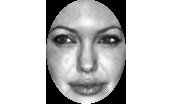
\includegraphics[width=\textwidth]{angelina/Angelina_Jolie_0006_CLAHE}
                \caption{CLAHE}
                \label{fig:clahe}
        \end{subfigure}
        %
        
        \begin{subfigure}[b]{0.2\textwidth}
                \centering
                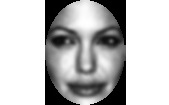
\includegraphics[width=\textwidth]{angelina/Angelina_Jolie_0006_gaussian}
                \caption{Gaussian}
                \label{fig:gaussian} 
        \end{subfigure}
        ~ ~
        \begin{subfigure}[b]{0.2\textwidth}
                \centering
                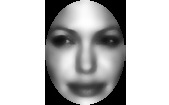
\includegraphics[width=\textwidth]{angelina/Angelina_Jolie_0006_bilateral}
                \caption{Bilateral}
                \label{fig:bilateral}
        \end{subfigure}
        ~ ~
        \begin{subfigure}[b]{0.2\textwidth}
                \centering
                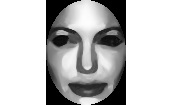
\includegraphics[width=\textwidth]{angelina/Angelina_Jolie_0006_akf}
                \caption{AKF}
                \label{fig:akf}
        \end{subfigure}
        \caption{Variação da mesma imagem nas várias galerias pré-processadas.}
        \label{fig:galeriaspreprocessadas}   
\end{figure}

\subsection{Avaliação \textit{Closed-set Identification}} \label{sec:avaliacao1}
O paradigma \textit{closed-set identification} é um método padrão de avaliação do desempenho de sistemas de reconhecimento facial automático, tendo sido utilizado, por exemplo, nas avaliações FERET \cite{Phillips2000} e FRVT \cite{BlackburnDuaneM.;BoneMike;Phillips2001}. Este paradigma corresponde a um sub-problema de identificação em que uma prova é apresentada ao sistema pretendendo-se que este devolva a identidade da pessoa presente na imagem. Neste caso particular do problema de identificação, todas as provas apresentadas possuem uma correspondência na galeria, em oposição ao caso geral de identificação, no qual pode ou não haver uma correspondência.

Para cada conjunto de teste descrito na Secção \ref{sec:conjuntos}, seja $\mathscr{G} = \{g_1, ..., g_N\}$ a sua galeria de treino, e seja $\mathscr{P} = \{p_1, ..., p_N\}$ o conjunto das suas provas. Quando uma prova $p_j$ é apresentada ao sistema, essa prova é comparada com cada amostra biométrica $g_i$ da galeria, resultando dessa comparação a respetiva medida de similaridade (\textit{similarity score}), $s_{ij}$. Esta medida é designada de $match$ $score$, caso $g_i$ e $p_j$ sejam amostras da mesma pessoa, caso não o sejam é designado de $nonmatch$ $score$. Quanto menor a medida de similaridade, maior é a probabilidade das imagens comparadas pertencerem à mesma pessoa, sendo que o melhor valor possível para a medida de similaridade de um $match$ $score$ é zero. Na identificação de $p_j \in \mathscr{P}$, em primeiro lugar são calculados os índices de similaridade para todas as amostras na galeria $\mathscr{G}$, sendo posteriormente ordenados os seus resultados. O \textit{rank} de $p_j$, $r_{p_j}$, é igual a $n$, se o seu $match$ $score$ corresponde à enésima menor medida de similaridade. 

Na avaliação de um conjunto de teste é calculado o \textit{rank} de cada uma das suas provas. Considerando que $|C(n)|$ corresponde ao número de provas com \textit{rank} $n$, ou menor do que $n$, e que $|\mathscr{P}|$ corresponde ao número de provas existentes em $\mathscr{P}$, a taxa de identificação para o \textit{rank} $n$, $T_{I}(n)$, corresponde à fração de provas com \textit{rank} $n$ ou menor do que $n$, ou seja:
\begin{equation}
T_{I}(n) = \frac{|C(n)|}{|\mathscr{P}|} \times 100
\end{equation}
A $T_{I}(n)$ é calculada para cada um dos \textit{ranks} de 1 a 30. Cada galeria é avaliada com os três algoritmos disponíveis, nos quatro conjuntos de teste sendo posteriormente calculada a média dos resultados obtidos para essa galeria. Os resultados apresentados de seguida correspondem à média dos resultados obtidos e encontram-se aqui reportados num conjunto de três experiências, cada uma dedicada a analisar a variação do comportamento do sistema dado um problema específico.

\subsubsection{Experiência 1: Impacto Segmentação das Faces.}

A primeira experiência realizada visa analisar o impacto da deteção e posterior segmentação das faces presentes numa imagem. Nesta experiência foram utilizadas as galerias de imagens Original, Cropped e Masked. A primeira é constituída pelas imagens originais da biblioteca LFW-a e permite estabelecer uma base de comparação entre as imagens segmentadas e as imagens originais. A galeria Cropped é composta por um conjunto de imagens onde as faces foram detetadas e segmentadas pelo detetor facial implementado no sistema Visage. A terceira e última galeria criada possui as mesmas imagens da galeria Cropped, sobre as quais foi posteriormente aplicada uma máscara elíptica de modo a aumentar a área de fundo removida das imagens recortadas. Os resultados obtidos no âmbito desta experiência encontram-se sintetizados na Tabela \ref{tab:media_exp1}.
\begin{table}
	\centering
    \caption{Média dos resultados obtidos nos 4 conjuntos de teste para as galerias Original, Cropped e Masked na Experiência 1 (melhores a negrito).}
	\begin{tabular}{c|>{\centering\arraybackslash}p{1.1cm}>{\centering\arraybackslash}p{1.1cm}>{\centering\arraybackslash}p{1.1cm}|>{\centering\arraybackslash}p{1.1cm}>{\centering\arraybackslash}p{1.1cm}>{\centering\arraybackslash}p{1.1cm}|>{\centering\arraybackslash}p{1.1cm}>{\centering\arraybackslash}p{1.1cm}>{\centering\arraybackslash}p{1.1cm}}
	~&\multicolumn{3}{c}{\textit{Eigenfaces}}&\multicolumn{3}{c}{\textit{Fisherfaces}}&\multicolumn{3}{c}{\textit{LBPH}}\\
	Rank & Orig. & Crop. & Mask. & Orig. & Crop. & Mask & Orig. & Crop. & Mask \\ 
	\hline\hline
	1 & 12.9\% & 25.9\% & 28.1\% & 30.1\% & 44.2\% & 43.6\% & 7.6\% & \textbf{47.3\%} & 46.8\% \\
	5 & 31.9\% & 50.0\% & 52.8\% & 58.8\% & 66.3\% & 66.5\% & 21.6\% & 70.8\% & \textbf{71.9\%} \\
	10 & 47.6\% & 64.0\% & 65.8\% & 71.3\% & 76.6\% & 75.3\% & 34.1\% & 79.8\% & \textbf{79.9\%} \\
	15 & 57.7\% & 72.9\% & 75.0\% & 80.6\% & 81.7\% & 81.0\% & 43.9\% & \textbf{87.1\%} & 85.8\% \\
	20 & 65.2\% & 81.3\% & 81.5\% & 86.4\% & 86.4\% & 84.4\% & 53.8\% & \textbf{90.4\%} & 90.2\% \\
	25 & 72.0\% & 86.2\% & 86.1\% & 90.2\% & 90.2\% & 88.6\% & 63.5\% & 92.4\% & \textbf{93.0\%} \\
	30 & 78.4\% & 89.5\% & 89.3\% & 92.2\% & 92.5\% & 91.0\% & 92.3\% & 94.0\% & \textbf{95.0\%} \\
	\hline\hline
    \end{tabular}
    \label{tab:media_exp1}
\end{table}

\subsubsection{Experiência 2: Impacto da Normalização do Contraste.}

A aquisição de imagens em condições não controladas pode resultar na obtenção de fotografias com um contraste reduzido e níveis de iluminação muito distintos. De forma a ultrapassar este problema, a normalização do contraste de uma imagem é uma tarefa comum nos sistemas de reconhecimento facial. Nesta experiência pretendemos analisar qual o impacto da normalização do contraste de uma imagem nos diferentes algoritmos avaliados, assim como determinar qual a melhor estratégia de normalização, de entre três técnicas implementadas, através da análise do desempenho do sistema nas galerias Normalized, onde foi aplicada a téncnica \textit{Contrast Stretching}; Equalized, onde foi efetuada a Equalização do Histograma; e Clahe, onde foi utilizada a técnica homónima. Os resultados obtidos no âmbito desta experiência encontram-se sintetizados na Tabela \ref{tab:media_exp2}.

\begin{table}
   	\centering
    \caption{Média dos resultados obtidos nos 4 conjuntos de teste para as galerias Normalized, Equalized e Clahe na Experiência 2 (melhores a negrito).}
	\begin{tabular}{c|>{\centering\arraybackslash}p{1.1cm}>{\centering\arraybackslash}p{1.1cm}>{\centering\arraybackslash}p{1.1cm}|>{\centering\arraybackslash}p{1.1cm}>{\centering\arraybackslash}p{1.1cm}>{\centering\arraybackslash}p{1.1cm}|>{\centering\arraybackslash}p{1.1cm}>{\centering\arraybackslash}p{1.1cm}>{\centering\arraybackslash}p{1.1cm}}
	~&\multicolumn{3}{c}{\textit{Eigenfaces}}&\multicolumn{3}{c}{\textit{Fisherfaces}}&\multicolumn{3}{c}{\textit{LBPH}}\\
	Rank & Norm. & Equa. & Clahe. & Norm. & Equa. & Clahe & Norm. & Equa. & Clahe \\ 
	\hline\hline
	1 & 30.0\% & 43.0\% & 40.9\% & 42.2\% & 47.3\% & 45.8\% & 45.7\% & \textbf{49.1\%} & 46.1\% \\
	5 & 56.7\% & 68.3\% & 68.0\% & 67.5\% & 67.5\% & 66.8\% & 70.6\% & \textbf{71.8\%} & 68.3\% \\
	10 & 70.4\% & 77.9\% & 80.3\% & 75.1\% & 77.5\% & 77.7\% & \textbf{80.9\%} & 80.3\% & 79.5\% \\
	15 & 79.7\% & 84.3\% & 86.8\% & 81.1\% & 83.7\% & 83.3\% & \textbf{87.3\%} & 85.6\% & 86.4\% \\
	20 & 85.0\% & 89.3\% & 90.6\% & 85.3\% & 87.1\% & 87.7\% & \textbf{91.0\%} & 89.3\% & 90.8\% \\
	25 & 89.4\% & 91.4\% & 93.4\% & 88.5\% & 89.1\% & 89.7\% & \textbf{94.0\%} & 92.4\% & 93.3\% \\
	30 & 92.3\% & 94.0\% & 95.0\% & 91.3\% & 91.1\% & 91.5\% & \textbf{95.7\%} & 94.2\% & 95.6\% \\
	\hline\hline
    \end{tabular}
    \label{tab:media_exp2}
\end{table}

\subsubsection{Experiência 3: Impacto da Abstração de Imagens.}

A terceira e última experiência realizada visa analisar qual o impacto da utilização de filtros de abstração no processo de reconhecimento facial em imagens. A análise foi efetuada com recurso a três filtros de abstração, gaussiano, bilateral e Kuwahara anisotrópico, os quais correspondem a diferentes técnicas e níveis de abstração, sendo o filtro gaussiano o filtro com um menor impacto na imagem original e o filtro Kuwahara anisotróprico aquele que produz um maior grau de abstração. Os resultados obtidos no âmbito desta experiência encontram-se sintetizados na Tabela \ref{tab:media_exp2}.

\begin{table}
	\centering
    \caption{Média dos resultados obtidos nos 4 conjuntos de teste para as galerias Gaussian, Bilateral e AKF na Experiência 3 (melhores a negrito).}
	\begin{tabular}{c|>{\centering\arraybackslash}p{1.1cm}>{\centering\arraybackslash}p{1.1cm}>{\centering\arraybackslash}p{1.1cm}|>{\centering\arraybackslash}p{1.1cm}>{\centering\arraybackslash}p{1.1cm}>{\centering\arraybackslash}p{1.1cm}|>{\centering\arraybackslash}p{1.1cm}>{\centering\arraybackslash}p{1.1cm}>{\centering\arraybackslash}p{1.1cm}}
	~&\multicolumn{3}{c}{\textit{Eigenfaces}}&\multicolumn{3}{c}{\textit{Fisherfaces}}&\multicolumn{3}{c}{\textit{LBPH}}\\
	Rank & Gaus. & Bila. & AKF. & Gaus. & Bila. & AKF & Gaus. & Bila. & AKF \\ 
	\hline\hline
	1 & 43.4\% & 42.7\% & 41.0\% & 44.4\% & 44.2\% & 42.7\% & \textbf{47.5\%} & 42.3\% & 31.5\% \\ 
	5 & 68.5\% & 67.9\% & 66.1\% & 64.8\% & 67.4\% & 66.4\% & \textbf{69.4\%} & 66.3\% & 56.6\% \\ 
	10 & 78.3\% & 77.7\% & 76.4\% & 75.6\% & 76.8\% & 77.9\% &\textbf{80.0\%} & 78.4\% & 67.3\% \\ 
	15 & 85.0\% & 85.1\% & 83.4\% & 81.7\% & 81.1\% & 83.7\% & \textbf{86.3\%} & 83.3\% & 74.1\% \\ 
	20 & 89.4\% & 89.7\% & 88.5\% & 85.0\% & 86.0\% & 86.9\% & \textbf{90.7\%} & 86.6\% & 81.4\% \\ 
	25 & 91.7\% & 91.8\% & 91.2\% & 88.7\% & 89.0\% & 91.4\% & \textbf{93.3\%} & 89.0\% & 85.0\% \\ 
	30 & 94.4\% & 94.5\% & 94.3\% & 91.5\% & 91.3\% & 94.2\% & \textbf{95.7\%} & 92.1\% & 87.9\% \\
	\hline\hline
    \end{tabular}
    \label{tab:media_exp3}
\end{table}

\subsection{Avaliação \textit{Image Retrieval}} \label{sec:avaliacao2}
Em recuperação de informação designa-se \textit{precisão} a fração de resultados relevantes do total de resultados retornados por uma pesquisa. No sistema de reconhecimento facial criado, para uma imagem fornecida é apresentada uma lista de possíveis entidades que se encontram representadas nessa imagem, em que o primeiro resultado representa a entidade com maior probabilidade de estar presente na imagem e em que cada entidade aparece uma única vez na lista de resultados. Caso se pretenda efetuar a identificação de uma personalidade existe apenas um resultado relevante na lista de resultados obtida. Ao analisar o desempenho do sistema torna-se importante verificar a posição em que surgem os resultados relevantes e não apenas a fração de resultados relevantes analisada pela \textit{precisão}.

\begin{table}[t]
	\centering
    \caption{Resultados da Média da Precisão na Galeria (melhores a negrito).}
    \begin{tabular}{l|ccc}
    Galeria    & $MPG_{Eigenfaces}$ & $MPG_{Fisherfaces}$ & $MPG_{LBPH}$ \\ 
    \hline\hline
    Original   & 23.1\%          & \textbf{43.4\%}  & 16.0\%             \\

    Cropped    & 37.7\%          & 54.8\%           & \textbf{58.2\%}    \\
    Masked     & 40.0\%          & 54.0\%           & \textbf{58.3\%}    \\

    Normalized & 42.4\%          & 53.5\%           & \textbf{57.2\%}    \\
    Equalized  & 55.2\%          & 57.3\%           & \textbf{59.6\%}    \\
    CLAHE      & 53.6\%          & 55.9\%           & \textbf{56.5\%}    \\

    Gaussian   & 55.3\%          & 54.2\%           & \textbf{58.1\%}    \\
    Bilateral  & 54.6\%          & \textbf{54.7\%}           & 53.8\%    \\
    AKF        & 52.8\%          & \textbf{53.9\%}           & 43.0\%             \\
    \hline\hline
    \end{tabular}
    \label{tab:resultadosprecicao}
\end{table}

Para avaliação do desempenho do sistema do ponto de vista de \textit{image retrieval} foi criada a medida \textit{precisão na galeria} (PG). A \textit{precisão na galeria} resulta da adaptação da precisão ao caso particular do sistema de reconhecimento facial automático desenvolvido. Considerando a definição de \textit{rank} de uma prova apresentada na Secção \ref{sec:avaliacao1}, seja $\mathscr{P}$ o conjunto de provas da galeria, $p_j \in \mathscr{P}$ e $r_{p_j}$ o \textit{rank} da prova $p_j$. A \textit{precisão na galeria} de $p_j$, $PG_{p_j}$, é definida como:
\begin{equation}
PG_{p_j} = \frac{1}{r_{p_j}} \times 100
\end{equation}
A \textit{precisão na galeria} é uma precisão no sentido em que é uma razão entre número de documentos relevantes (aqui sempre 1) e número de documentos na resposta. Nesta avaliação o que consideramos é uma resposta de tamanho variável e igual ao número de amostras que é necessário considerar até incluir a relevante. A \textit{precisão na galeria} é maior quanto mais cedo o nome da pessoa a identificar aparece na lista de resultados possíveis. Por outro lado, a distância entre precisões na galeria sucessivas é maior quanto maior forem os valores de precisão. Como tal, é possível efetuar uma análise do desempenho do sistema com ênfase nos resultados de topo, ao mesmo tempo que se diferenciam os valores de precisão mais elevados, os quais representam os resultados mais significativos para os utilizadores do sistema.

A análise do desempenho de um algoritmo é efetuada com recurso à análise do seu desempenho para um conjunto de provas. Seja $n$ o número de provas existentes em $\mathscr{P}$, a \textit{média da precisão na galeria} (MPG) de um algoritmo é calculada através da média da \textit{precisão na galeria} obtida para cada prova e pode ser definida como:
\begin{equation}
MPG_{algoritmo} = \frac{ \sum\limits_{i=0}^{n} PG_{p_i} }{n}
\end{equation}

A \textit{média da precisão na galeria} para as nove galerias avaliadas encontra-se reportada na Tabela \ref{tab:resultadosprecicao}.


\section{Requisitos Armazenamento}
Um sistema de reconhecimento facial automático pode ser analisado do ponto de vista do seu desempenho no reconhecimento, no entanto, as necessidades de processamento e armazenamento das imagens utilizadas por este tipo de sistemas devem também ser objeto de análise. 

Na Tabela \ref{tab:tamanho} encontram-se sintetizadas as necessidades de armazenamento das imagens que compõem as galerias utilizadas na avaliação do sistema Visage. Todas as galerias pré-processadas reduzem em pelo menos 81\% as necessidades de armazenamento necessárias. A este nível as imagens da galeria AKF, abstraídas com recurso ao filtro Kuwahara anisotrópico, destacam-se uma vez que são em média 89\% inferiores às imagens originais. A redução do espaço de armazenamento com recurso à abstração permite a criação de galerias mais fáceis e rápidas de processar pelo sistema, ao mesmo tempo que reduz da quantidade de dados transferidos na utilização do sistema Visage em cooperação com eventuais clientes web ou aplicação móveis.
\begin{table}
	\centering
    \caption{Necessidades de armazenamento galerias pré-processadas.}
    \begin{tabular}{l|ccccc}
    Galeria    & Total(MB) & Médio (KB) & Máximo (KB) & Mínimo (KB) & Diferença \\ 
    \hline\hline
    Original   & 125.5   & 81 & 114 & 47 & - \\

    Cropped    & 20.9   & 13 & 18 & 9 & -83.4\% \\
    Masked     & 19.4   & 12 & 16 & 9 & -84.5\% \\  

    Normalized & 20.7   & 13 & 16 & 10& -83.5\% \\  
    Equalized  & 23.7   & 15 & 18 & 12& -81.1\% \\  
    CLAHE      & 22.9   & 15 & 18 & 12& -81.7\% \\  

    Gaussian   & 22.4   & 14 & 17 & 12& -82.2\% \\  
    Bilateral  & 21.7   & 14 & 16 & 11& -82.7\% \\  
    AKF        &\textbf{ 13.7}   & \textbf{9}  & \textbf{11} & \textbf{6} & \textbf{-89.1\%} \\  
    \hline\hline
    \end{tabular}
    \label{tab:tamanho}
\end{table}
\section{Discussão e Conclusão}
Neste artigo avaliamos o sistema de reconhecimento facial Visage ao nível do seu desempenho no reconhecimento, e também ao nível dos requisitos de armazenamento necessários utilizando nove cadeias de pré-processamento de imagens.

As avaliações efetuadas permitem concluir que a etapa de pré-processamento que permite um maior aumento no número de indivíduos corretamente reconhecidos é a deteção e segmentação das faces presentes numa imagem. Através da comparação do desempenho das galerias Original, Cropped e Masked é ainda possível concluir que a segmentação da face da restante imagem produz um maior impacto no algoritmo \textit{LBPH}, seguido pelo algoritmo \textit{Fisherfaces} e em último lugar pelo algoritmo \textit{Eigenfaces}. Finalmente, a este nível é ainda possível destacar que não se registou uma diferença significativa no desempenho do sistema entre as imagens com máscara e as imagens apenas recortadas. A aplicação de uma máscara constitui, no entanto, uma técnica tipicamente aplicada para a remoção de uma maior quantidade de fundo das imagens \cite{Phillips2000,ahonen2004face,Kumar2009}, uma vez que permite obter uma maior confiança nos resultados obtidos ao garantir que o reconhecimento efetuado não tira partido dos elementos existentes no fundo da imagens, mas sim das caraterísticas faciais representadas \cite{Kumar2009}.

Ao nível da normalização do contraste das imagens verificou-se que a aplicação desta etapa de pré-processamento permite uma melhoria no número de faces corretamente reconhecidas, com particular ênfase no algoritmo \textit{Eigenfaces}, onde se registou uma melhoria de 15,2\% na comparação da \textit{média da precisão na galeria} das galerias Equalized e Masked. Na comparação das três técnicas de normalização do contraste, a equalização simples do histograma e a técnica \textit{CLAHE} foram as que revelaram melhores resultados para os algoritmos \textit{Eigenfaces} e \textit{Fisherfaces}. No caso algoritmo \textit{LBPH}, a técnica de \textit{Contrast Stretching} e a equalização simples do histograma revelaram os melhores resultados. Contudo, a equalização do histograma demonstrou um desempenho ligeiramente superior na taxa de identificação para os primeiros \textit{ranks}, tendo sido por isso utilizada como técnica de normalização na cadeia de pré-processamento das imagens abstraídas. A reduzida diferença no desempenho das galerias Normalized, Equalized e CLAHE justifica um estudo mais aprofundado das técnicas de normalização do contraste em trabalho futuro.

Por último, a avaliação efetuada à utilização de abstração de imagens no âmbito do processo de reconhecimento facial automático revela a existência de um compromisso entre a redução das necessidades de armazenamento das imagens abstraídas e uma ligeira diminuição do desempenho do reconhecimento efetuado. A este nível destaca-se a utilização do filtro Kuwahara anisotrópico para a abstração das imagens, o qual permite uma redução de 89\% do espaço de armazenamento, implicando no entanto uma diminuição de cerca de 6\% na \textit{média da precisão da galeria} quando comparadas as galerias AKF e Equalized. A aplicação da abstração com recurso aos filtros gaussiano e bilateral demonstrou um menor impacto no desempenho do reconhecimento, mas também uma menor redução nos requisitos de armazenamento das respetivas galerias. Este fator pode ser explicado devido à maior semelhança entre as imagens abstraídas com recurso a estes filtros e as imagens não abstraídas, devido ao menor grau de abstração por eles aplicado. A combinação da galeria Gaussian com a utilização do algoritmo \textit{LBPH} obteve a taxa de identificação mais elevada das galerias abstraídas, sendo esta, no entanto, ligeiramente inferior às taxas de identificação mais elevadas das galerias utilizadas na Experiência 2. 

\bibliography{myrefs}
\bibliographystyle{splncs}
\end{document}